% =====================================================================
%  c05 —— PDF p.39–45（原书 p.33–39）
%  §2.4 二次微分的存在定理
% =====================================================================

% ===== 原书 p.33 =====
% （本页开头承接上一块：定理 2.4 陈述的末段，由 c04 译完，此处跳过；
%   以下从本页开始的定理 2.4 的证明起译。）

\begin{proof}
设$a_i$为$R_i$的长度，$\varphi$为把$R_i'$映到$R=\{z\mid\exp(-2\pi iM_i')<|z|<1\}$的正则映射。再考虑$\frac{b_i}{2\pi iM_i}\log(\varphi)$，它把$R_i'$映到$S_i'=\{x+iy\mid0<x<\tilde a_i,\ 0<y<b_i\}$，其中$\tilde a_i=\frac{b_i}{M_i}$。这里写成$|\sqrt{\omega}|=\rho(x,y)\sqrt{dx^2+dy^2}$时，由
\[
a_i\le\int_0^{\tilde a_i}\rho(x,y)\,dx
\]
得
\[
a_ib_i\le\int_{S_i'}\rho(x,y)\,dx\,dy,\qquad
\sum_{i=1}^n a_ib_i\le\sum_{i=1}^n\int_{S_i'}\rho(x,y)\,dx\,dy.
\]
因此
\[
\begin{aligned}
\left(\sum_{i=1}^n a_ib_i\right)^2
&\le\left(\sum_{i=1}^n\int_{S_i'}\rho(x,y)\,dx\,dy\right)^2\\
&\le\left(\sum_{i=1}^n\tilde a_ib_i\right)
 \left(\sum_{i=1}^n\frac{1}{\tilde a_ib_i}
 \left(\int_{S_i}\rho(x,y)\,dx\,dy\right)^2\right)\\
&\le\left(\sum_{i=1}^n\tilde a_ib_i\right)
 \left(\sum_{i=1}^n\frac{1}{\tilde a_ib_i}
 \int_{S_i}\rho^2(x,y)\,dx\,dy\cdot\tilde a_ib_i\right)\\
&=\left(\sum_{i=1}^n\tilde a_ib_i\right)
 \left(\sum_{i=1}^n\int_{S_i}\rho^2(x,y)\,dx\,dy\right)\\
&\le\left(\sum_{i=1}^n\tilde a_ib_i\right)
 \left(\sum_{i=1}^n a_ib_i\right).
\end{aligned}
\]
由此得到$\sum_{i=1}^n a_ib_i\le\sum_{i=1}^n\tilde a_ib_i$。等号的情形与引理 2.2 相同，故省略。
\end{proof}

\transnote{原书 p.33 的证明开头把环域写作$\exp(-2\pi iM_i')<|z|<1$，把映射的分母写作$2\pi iM_i$；其中$i$的用法以及$M_i$与$M_i'$的搭配疑有笔误，此处照原文译出。}

\subsection{二次微分的存在定理}

\begin{theorem}
设$X$为 Riemann 面，$\gamma_1,\dots,\gamma_n$为可容许（admissible）的曲线系。假设条件
% ===== 原书 p.34 =====
\begin{itemize}[leftmargin=3.2em,itemsep=2pt,topsep=4pt]
\item[(fin)] 集合$\{M_i\mid M_i$为与$\gamma_i$同伦等价的环域$R_i$的模$\}$有界
\end{itemize}
成立。则对$\R_+$中任意元素$b_1,\dots,b_n$，存在唯一的二次微分$\omega$，它具有类型$(\gamma_i)_i$的闭轨道，且以$b_1,\dots,b_n$为特征环域（characteristic ring domain）的高度。
\end{theorem}

\begin{proof}
取互不相交的类型$(\gamma_i)_i$的环域$(R_{ip})$（$p=1,2,\dots$），设$M_{ip}$为$R_{ip}$的模，并使$\sum_{i=1}^n\frac{b_i^2}{M_{ip}}$成为趋于其下确界的序列。因$M_i$有界，故必要时取其部分列，可设$\lim_{p\to\infty}M_{ip}=M_i$存在。设$g_{in}$为从$D_{in}=\{\exp(-2\pi M_{in})<|z|<1\}$到$R_{in}$的正则同构，则利用正规族的论述，作为$\{g_{in}\}_n$的某个部分列的极限，存在从$D_i=\{\exp(-2\pi M_i)<|z|<1\}$到$X$的函数$g_i$；其像$R_i$为互不相交的类型$(\gamma_i)_i$的环域，且$\sum_{i=1}^n\frac{b_i^2}{M_i}$达到前面出现的下确界。

现考虑与 id 充分「接近」的$C^\infty$-map $F\colon R\to R$。（所谓「接近」，后面会明白。）记$\tilde R_i=F(R_i)$，$R_i,\tilde R_i$的模分别为$M_i,\tilde M_i$。设$R_i,\tilde R_i$与$D_{M_i},D_{\tilde M_i}$的同构为$\varphi,\tilde\varphi_i$，$a_i=\frac{b_i}{M_i}$，$\tilde a_i=\frac{b_i}{\tilde M_i}$。这里$D_M=\{z\in\C\mid\exp(-2\pi M)<|z|<1\}$。

\transnote{原文把 $C^\infty$ 映射写作「$C^\infty$-map」（原书 p.34），下文（原书 p.35）亦同；译本照原文保留该写法，不改为「映射」。}

再令$\zeta=\frac{a_i}{2\pi i}\log\varphi_i$，$f(\zeta)=\frac{\tilde a_i}{2\pi i}\log\tilde\varphi_i$。此时作为$\zeta$的函数，$f(\zeta)$只能确定到相差$2\pi i\Z$，但$f_\zeta=\frac{df}{d\zeta}$、$f_{\bar\zeta}=\frac{df}{d\bar\zeta}$确定；由$\zeta=\xi+i(\text{const.})$确定的曲线族经$f$的像的长度，可用$\int|f_\zeta+f_{\bar\zeta}|\,d\xi$计算。因此
\[
\tilde a_i\le\int|f_\zeta+f_{\bar\zeta}|\,d\xi
\]
成立。令$\zeta=\xi+\eta i$，在$S_i$上进行上面的积分，则
\[
\begin{aligned}
\tilde a_ib_i&\le\int_{S_i}|f_\zeta+f_{\bar\zeta}|\,d\xi\,d\eta\\
&=\int J(f)^{\frac12}\,\frac{|f_\zeta+f_{\bar\zeta}|}{J(f)^{\frac12}}\,d\xi\,d\eta
\end{aligned}
\]
成立。这里利用$J(f)=|f_\zeta|^2-|f_{\bar\zeta}|^2$，由 Schwarz 不等式得
\[
\begin{aligned}
(\tilde a_ib_i)^2&\le\int_{S_i}J\,d\xi\,d\eta\int_{S_i}
 \frac{|f_\zeta+f_{\bar\zeta}|^2}{|f_\zeta|^2-|f_{\bar\zeta}|^2}\,d\xi\,d\eta\\
&=\tilde a_ib_i\int_{S_i}\frac{|1+\kappa|^2}{1-|\kappa|^2}\,d\xi\,d\eta.
\end{aligned}
\]

% ===== 原书 p.35 =====
这里$\kappa=f_{\bar\zeta}/f_\zeta$，是称为伸缩率（dilatation）的数。因此
\[
\frac{b_i^2}{\tilde M_i}\le\int_{S_i}\frac{|1+\kappa|^2}{1-|\kappa|^2}\,d\xi\,d\eta\qquad(\ast)
\]
成立。

现设$U$为$X$的充分小的开集，$z=x+yi$为$U$上的复坐标。又设$h(z)$为$U$上具有充分小支集的$C^\infty$函数。此时对充分小的$\epsilon$，$F\colon z\mapsto z+\epsilon h(z)$是$U$上的微分同胚，并在$U$以外延拓为 id。令$U_i=U\cap R_i$，就这个$F$执行$(\ast)$的积分。设$\Phi_i=\frac{a_i}{2\pi i}\log\varphi_i\colon R_i\to S_i$，$W_i$为对应于$U_i$的开集，注意在$S_i-W_i$上为 id 且$\kappa=0$，则
\[
\begin{aligned}
\int_{S_i}\frac{|1+\kappa|^2}{1-|\kappa|^2}\,d\xi\,d\eta
&=\int_{S_i-W_i}d\xi\,d\eta+\int_{W_i}\frac{|1+\kappa|^2}{1-|\kappa|^2}\,d\xi\,d\eta\\
(\ast\ast)\qquad
&=\int_{S_i-W_i}d\xi\,d\eta+\int_{U_i}\frac{|1+\kappa|^2}{1-|\kappa|^2}
 \left|\frac{d}{dz}\Phi_i\right|^2dx\,dy
\end{aligned}
\]
成立。

第2项的积分要用伸缩率的性质。一般地，伸缩率$\kappa$是对复区域$D_1,D_2$、与共形等价充分接近的$C^\infty$-map $f\colon D_1\to D_2$、以及$D_1,D_2$的单值化参数（uniformizer）$z_1,z_2$定义的量，由
\[
\kappa=\kappa(f,z_1,z_2)
=\left(\frac{\partial(z_2\circ f)}{\partial\bar z_1}\right)
\Big/\left(\frac{\partial(z_2\circ f)}{\partial z_1}\right)
\]
定义。容易看出，它不依赖于$D_2$的单值化参数$z_2$。又容易看出，把$z_1$换成别的单值化参数$z_1'$时，令$\tau=\frac{dz_1'}{dz_1}$，有
\[
\kappa(f,z_1',z_2)=\kappa(f,z_1,z_2)\cdot\frac{\tau}{\bar\tau}
\]
成立。上面给出的$F$关于$z$坐标的伸缩率为$\frac{\epsilon h_{\bar z}(z)}{1+\epsilon h_z(z)}$，故关于$\zeta$的伸缩率为
\[
\frac{\epsilon h_{\bar z}(z)}{1+\epsilon h_z(z)}
\cdot\frac{\left(\frac{d}{dz}\Phi_i\right)^2}
{\left|\frac{d}{dz}\Phi_i\right|^2}.
\]
$(\ast\ast)$第2项的被积函数在模$O(\epsilon^2)$的意义下等于
\[
\begin{aligned}
\frac{|1+\kappa|^2}{1-|\kappa|^2}\left|\frac{d}{dz}\Phi_i\right|^2
&=|1+\kappa|^2\left|\frac{d}{dz}\Phi_i\right|^2+O(\epsilon^2)\\
&=(1+2\Re(\kappa))\left|\frac{d}{dz}\Phi_i\right|^2+O(\epsilon^2)\\
&=\left|\frac{d}{dz}\Phi_i\right|^2
 +2\epsilon\Re\left(h_{\bar z}\left(\frac{d}{dz}\Phi_i\right)^2\right)+O(\epsilon^2).
\end{aligned}
\]

% ===== 原书 p.36 =====
因此$(\ast\ast)$的积分等于
\[
a_ib_i+2\epsilon\Re\int_{U_i}h_{\bar z}
\left(\frac{d}{dz}\Phi_i\right)dx\,dy+O(\epsilon^2)\text{。}
\]
由此
\[
\begin{aligned}
\sum_{i=1}^n a_ib_i&\le\sum_{i=1}^n\tilde a_ib_i\\
&\le\sum_{i=1}^n\left(a_ib_i+2\epsilon\Re\int_{U_i}h_{\bar z}
 \left(\frac{d}{dz}\Phi_i\right)^2dx\,dy\right)+O(\epsilon^2).
\end{aligned}
\]
由于充分小的$\epsilon$可任意变动，
\[
\sum\Re\int_{U_i}h_{\bar z}
\left(\frac{d}{dz}\Phi_i\right)^2dx\,dy=0
\]
成立。

$h_{\bar z}$是具有充分小支集的任意$C^\infty$函数，故把各$U_i$上的$\left(\frac{d}{dz}\Phi_i\right)^2$粘贴所得的函数，作为广义函数看时关于$\bar z$的微分为$0$。因此它与$U$上某个全纯函数除一个零测集外一致。由此$\left(\frac{d}{dz}\Phi_i\right)^2dz^{\otimes2}$定义了$X$上的全纯二次微分。对应的特征环域为$R_i$。唯一性由定理 2.4 推出。
\end{proof}

\begin{remark}
用现在的方法，由$(b_1,\dots,b_n)$唯一确定$(M_1,\dots,M_n)$，但已知这个对应是连续的（Strebel）。后文也要用这个事实，证明省略。
\end{remark}

下面考察给定模时的情形。设给定 Riemann 面$X$与曲线的可容许系$\gamma_1,\dots,\gamma_n$，且定理 2.5 的条件 (fin) 满足。此时令
\[
\mathcal{H}=\Bigl\{(b_1^2,\dots,b_n^2)\ \Bigm|
\begin{array}{l}
\text{$X$上存在二次微分$\omega$，它满足$\|\omega\|_X=1$，具有类型$(\gamma_i)_i$的闭轨道，}\\[1pt]
\text{且关于$\gamma_1,\dots,\gamma_n$的特征环域的高度为$b_1,\dots,b_n$}
\end{array}\Bigr\}.
\]
称之为高度曲面（height surface）。现对$e=(e_1,\dots,e_n)$，$\sum e_i^2=1$，$e_i>0$，存在唯一的$\lambda>0$使$\lambda e\in\mathcal{H}$。事实上，取具有类型$(\gamma_i)_i$的闭轨道、对应特征环域的高度为$\sqrt{e_1},\dots,\sqrt{e_n}$的二次微分$\omega'$，令$\omega=\omega'/\|\omega'\|_X$，其高度记为$b_1,\dots,b_n$，则$(b_1^2,\dots,b_n^2)\in\mathcal{H}$，且
\[
(b_1^2,\dots,b_n^2)=(e_1,\dots,e_n)\cdot\|\omega'\|_X^{-2}
\]
成立。

% ===== 原书 p.37 =====
又由定理 2.5 的唯一性，若$\omega^{(1)},\omega^{(2)}$都具有类型$(\gamma_i)_i$的闭轨道，其特征环域的高度分别为$(b_1^{(1)},\dots,b_n^{(1)})$、$(b_1^{(2)},\dots,b_n^{(2)})$，且$\mu(b_1^{(1)},\dots,b_n^{(1)})=(b_1^{(2)},\dots,b_n^{(2)})$，则$\mu\omega^{(1)}=\omega^{(2)}$。在$\|\omega^{(1)}\|_X=\|\omega^{(2)}\|_X$的假设下，$\mu=1$，从而$\R_+e\cap\mathcal{H}$只有一点。

\begin{lemma}
$\mathcal{H}\subset\R^n$是严格凸的，在点$(x_1,\dots,x_n)=(b_1^2,\dots,b_n^2)$处的切平面由
\[
\frac{x_1}{M_1}+\cdots+\frac{x_n}{M_n}=1
\]
给出。这里$(M_1,\dots,M_n)$为对应于$(b_1^2,\dots,b_n^2)$的二次微分$\omega$的特征环域的模。
\end{lemma}

\begin{proof}
设$\tilde\omega$为具有类型$(\gamma_i)_i$的闭轨道、满足$\|\tilde\omega\|_X=1$、且其特征环域的高度为$\tilde b_1,\dots,\tilde b_n$的二次微分。此时只需证明
\[
\frac{\tilde b_1^2}{M_1}+\cdots+\frac{\tilde b_n^2}{M_n}\ge1.
\]
这是因为：当互不相交的类型$(\gamma_i)_i$的环域的模$m_i$变动时，使$\frac{\tilde b_1^2}{m_1}+\cdots+\frac{\tilde b_n^2}{m_n}$达到最小值的$(m_1,\dots,m_n)$，正是$\tilde\omega$的特征环域$\tilde R_i$的模$\tilde M_1,\dots,\tilde M_n$，故
\[
\frac{\tilde b_1^2}{M_1}+\cdots+\frac{\tilde b_n^2}{M_n}
\ge\frac{\tilde b_1^2}{\tilde M_1}+\cdots+\frac{\tilde b_n^2}{\tilde M_n}=1
\]
成立。又当等号成立时，令$R_i$为$\omega$的特征环域，则$\tilde R_i=R_i$。这意味着$\mathcal{H}$是严格凸的。
\end{proof}

\begin{center}
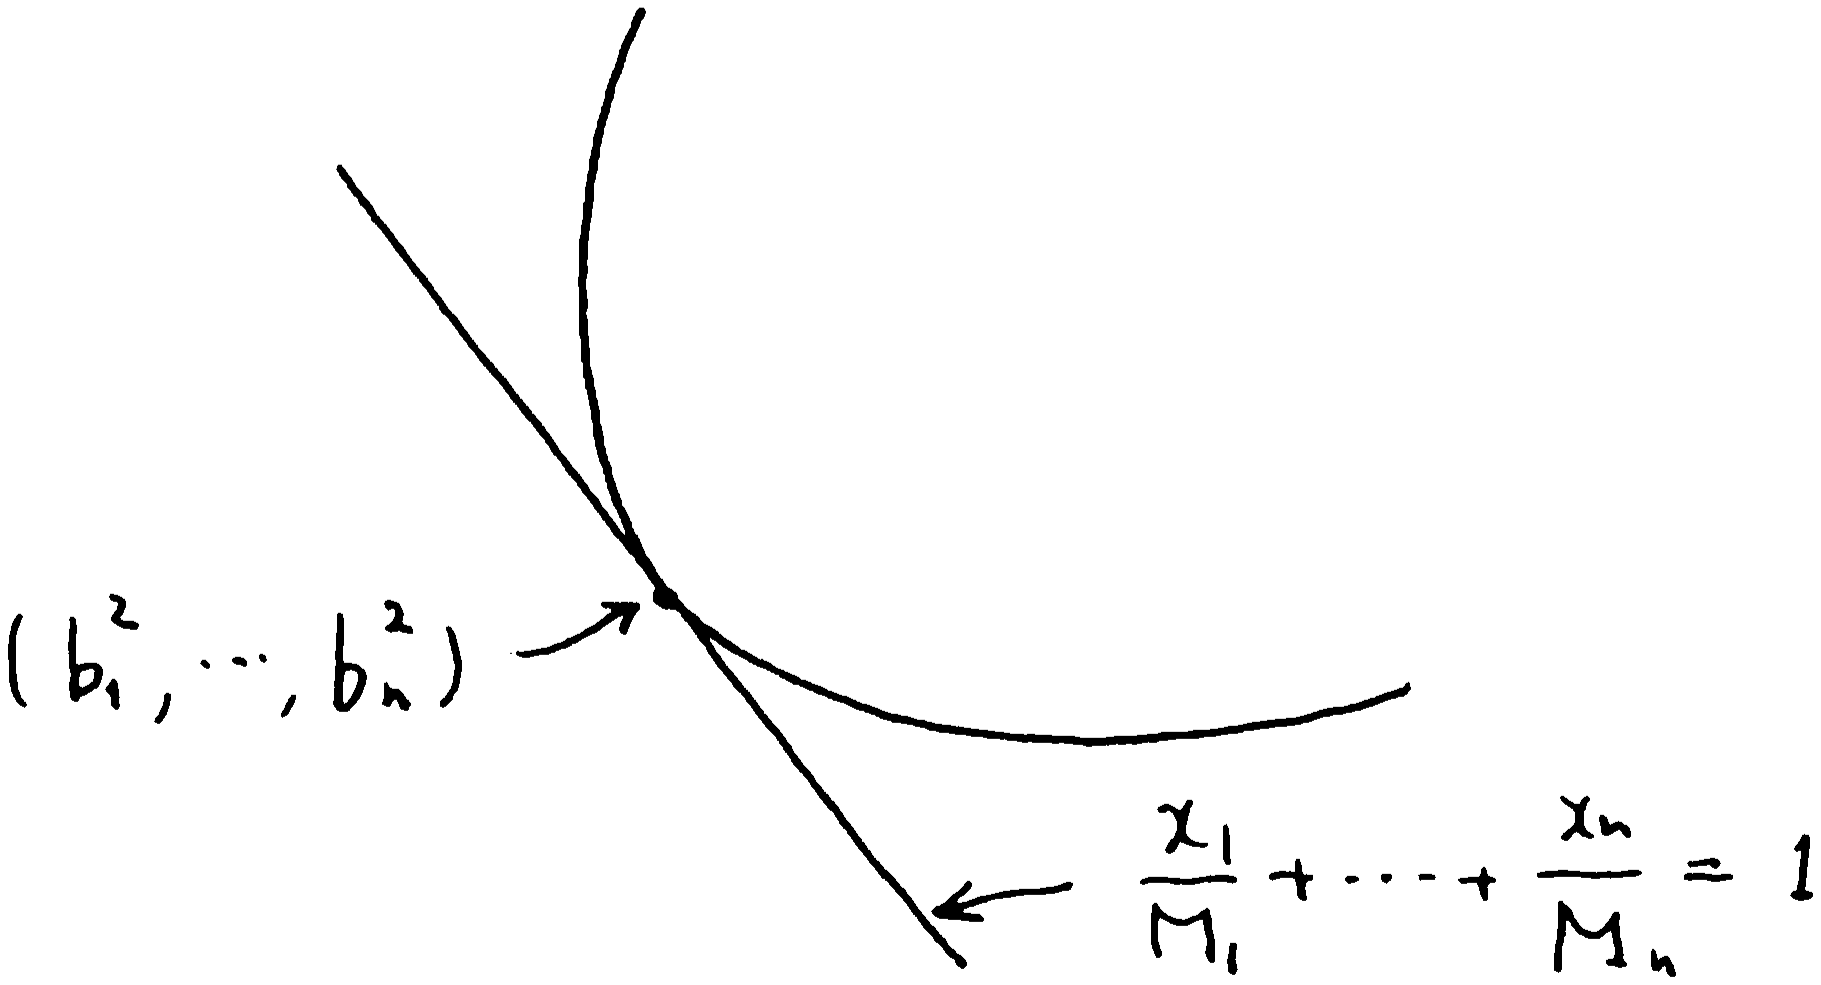
\includegraphics[width=0.5\linewidth]{fig_p43_a.png}
\end{center}

下面看看$\mathcal{H}$的边界上的情形。

% ===== 原书 p.38 =====
\begin{lemma}
\begin{enumerate}[label=(\arabic*)]
\item $\mathcal{H}$是有界集合。
\item 对$1\le i\le n$，考虑$\{x_i=0\}\cap\bar{\mathcal{H}}$。则对任意的
$e=(e_1,\dots,\check{0},\dots,e_n)$，$e_1^2+\cdots+e_n^2=1$，$e_i>0$，
存在某个$\lambda$使$\lambda e\in\{x_i=0\}\cap\bar{\mathcal{H}}$，
且该处的切平面的法向量由$(0,\dots,\check{1},\dots,0)$给出。
这里$\bar{\mathcal{H}}$是$\mathcal{H}$在$\R^n$内的闭包。
\end{enumerate}
\end{lemma}

\begin{proof}
(1) 由$\frac{\tilde b_1^2}{M_1}+\cdots+\frac{\tilde b_n^2}{M_n}=1$得$b_1^2\le M_1$，再由条件 (fin) 知有界。

(2) 考虑$b_i\to0$的极限，对$\gamma_1,\dots,\check{\gamma}_i,\dots,\gamma_n$考虑求高度为$b_1,\dots,\check{b}_i,\dots,b_n$的二次微分的问题，可知$M_i\to0$。切平面的法向量
\[
\left(\frac{1}{M_1},\dots,\frac{\check{1}}{M_i},\dots,\frac{1}{M_n}\right)
\Big/\sqrt{\sum_{i=1}^nM_i^{-2}}
\]
收敛于$e_i$。
\end{proof}

\transnote{原书 p.38 引理 2.7 的证明 (1) 处印作$b_1^2\le M_1$（只带下标$1$），据上下文应为$b_i^2\le M_i$；此处照原文印出。}

下面证明给定模（之比）时二次微分的存在性。

\begin{theorem}
设$X,(\gamma_i)_i$与定理中相同，并假设条件 (fin) 成立。给定$m=(m_1,\dots,m_n)\in\R_+^n$时，存在唯一的二次微分$\omega$，它满足$\|\omega\|_X=1$，具有类型$(\gamma_i)_i$的闭轨道，且其模$M_1,\dots,M_n$满足$(M_1,\dots,M_n)=\lambda(m_1,\dots,m_n)$（$\lambda>0$）。
\end{theorem}

\transnote{原书定理 2.8 的陈述只说「与 Theorem 相同」，未标编号，据前后文当指定理 2.5；此处照原文译出。}

\begin{proof}
令$e=(m_1,\dots,m_n)/\sqrt{\sum m_i^2}=(e_1,\dots,e_n)$，$c=\min\{x_1e_1+\cdots+x_ne_n\mid(x_1,\dots,x_n)\in\bar{\mathcal{H}}\}$。证明达到这个最小值的$(x_1,\dots,x_n)$属于$\R_+^n$。若不然，设$x=(t_1,\dots,\check{0},\dots,t_n)$，且这个$c$被达到。过此点、以$e$为法向量的平面为$e_1(x_1-t_1)+\cdots+e_ix_i+\cdots+e_n(x_n-t_n)=0$。若$(y_1,\dots,y_n)\in\bar{\mathcal{H}}$，则必须有$e_1(y_1-t_1)+\cdots+e_iy_i+\cdots+e_n(y_n-t_n)\ge0$。考虑满足$(y_1,\dots,\check{0},\dots,y_n)=\tau(t_1,\dots,t_n)$且$y_i\to t_i$的情形，则$(y_1-t_1:\cdots:y_i:\cdots:y_n-t_n)$收敛于与$e_i$正交的方向，因此$\frac{y_i}{1-\tau}\to0$。此时
\[
e_1(y_1-t_1)+\cdots+e_iy_i+\cdots+e_n(y_n-t_n)
=(\tau-1)e_1t_1+\cdots+e_iy_i+\cdots+(\tau-1)e_nt_n,
\]
故存在某个$(y_1,\dots,y_n)$使上式为负。这与前面矛盾。

% ===== 原书 p.39 =====
又，$c$的值在两个以上坐标变为$0$的点处被达到的情形也同样可证。（注意，思考其意义可知，把$\bar{\mathcal{H}}$限制到$x_i=0$上正是关于$\gamma_1,\dots,\check{\gamma}_i,\dots,\gamma_n$的高度曲面，因此考察只有一个坐标变为$0$的情形就足够了。）
\end{proof}
